\documentclass[../sparc.tex]{subfiles}
\graphicspath{{\subfix{../images/}}}
\begin{document}

%%%%%%%%%%%%%%%%%%%%%%%%%%%%%%%%%%%%%%%%%%%%%%%%%%%%%%%%%%%%%%%%%%%%%%%%%%%%%%%%
\section{Duty cycle}

How the voltage from the output range is set?  Pretty easy: by changing the
period of logical levels.  The more percentage of time the \texttt{HIGH} value
is supplied to the digital port, the higher the voltage.  In this case, the
length of the period \texttt{T} is kept fixed (e.g. to 1000 microseconds.)  Thus
for the \gls{PWM} to work the percentage relation of one logical level to
another is important; increasing the time of supplying one logical level we have
to decrease the time of another.

\example{
  If we supply the \texttt{HIGH} value for 60\% of the specified period
  \texttt{T}, we have fill the leftover 40\% percent of period with the
  \texttt{LOW} value.
}

The relation of signal period to the length of the impulse is known as the
\emph{duty cycle}.

\example{
  Let's say we want to get 2.5 Volts out of a digital port number 2.  We have
  only two logical values -- \texttt{LOW} (0V) and \texttt{HIGH} (5V.)  To solve
  the task we need to implement a PWM with 50\% duty cycle.  Thus in case of
  1000 $\mu\mbox{s}$ period \texttt{T} we have to set the port to \texttt{HIGH}
  for the half of \texttt{T} (500$\mu\mbox{s}$), and the rest of \texttt{T} we
  have to set the port to \texttt{LOW}.  If we do this right, then on the
  digital port number we will get 2.5 Volts.
}

For the PWM signal generation we have to implement a tool (a \emph{procedure})
that we will be using afterwards.  We have already talked about the importance
of creation and usage our own procedures in programs -- procedures allow us to
create modular programs, make it easier write new code and to maintain the
existing program code.

\begin{figure}[ht]
  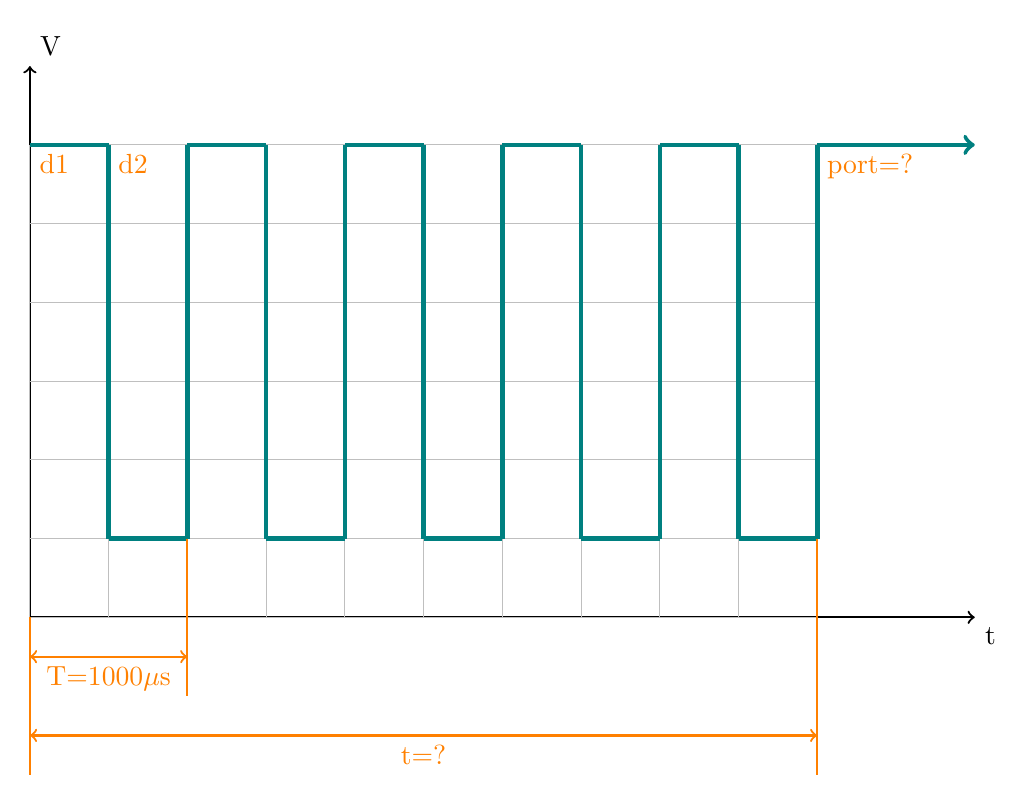
\begin{tikzpicture}
    \draw[thick, ->] (0, 0) -- (12, 0) node[anchor=north west] {t};
    \draw[thick, ->] (0, 0) -- (0,  7) node[anchor=south west] {V};
    \draw[lightgray] (0, 0) grid (10, 6);
    \foreach \x in {0, 2, ..., 8} {
      \draw[ultra thick, teal] (\x, 6) -- (\x + 1, 6);
      \draw[ultra thick, teal] (\x + 1, 6) -- (\x + 1, 1);
      \draw[ultra thick, teal] (\x + 1, 1) -- (\x + 2, 1);
      \draw[ultra thick, teal] (\x + 2, 1) -- (\x + 2, 6);
    }
    \draw[ultra thick, teal, ->] (10, 6) -- (12, 6);
    \draw[orange] (10, 6) node[anchor=north west] {port=?};
    \draw[orange] (0, 6) node[anchor=north west] {d1};
    \draw[orange] (1, 6) node[anchor=north west] {d2};
    \draw[thick, orange] (0,  0) -- (0,   -2);
    \draw[thick, orange] (2,  1) -- (2,   -1);
    \draw[thick, orange] (10, 1) -- (10,  -2);
    \draw[thick, orange, <->] (0, -0.5) -- (2,  -0.5)  node[midway, below] {T=1000$\mu\mbox{s}$};
    \draw[thick, orange, <->] (0, -1.5) -- (10,  -1.5) node[midway, below] {t=?};
  \end{tikzpicture}
  \caption{A graphical representation of the PWM signal generation.}
  \label{fig:pwm-graph}
\end{figure}

Let's think about the \gls{PWM} and how it could be implemented.  On the
fig. \ref{fig:pwm-graph} the PWM signal generation is shown in the form of a
graph.  We will be using this graph as the basis for writing our PWM procedure.

With this graph it is quite easy to lay down the description of the procedure in
natural language.  Let's call the procedure \texttt{pwm}, as the shorthand for
\emph{pulse-width modulation}.

We start from the fact that such procedure have to accept three parameters:

\begin{enumerate}
\item The port number (represented by an integer value) on which we have to
  generate a PWM signal; let's call this parameter just \texttt{port}.
\item The duty cycle (represented by a fraction value) that sets the output
  voltage on the \texttt{port} -- for example, the duty cycle of 50\% will be
  specified as 0.5.  Let's call this parameter \texttt{dc} (as the shorthand for
  ``duty cycle''.)
\item The duration of the PWM signal in microseconds.  Let's call this parameter
  \texttt{t} (as the shorthand of ``time''.)
\end{enumerate}

\end{document}
